\section{Prüfung 16.03.2022}
\subsection{Profit / Penalty}
Für die Reparatur eines wertvollen Oldtimer-Fahrzeugs wird dringend ein Ersatzteil benötigt welches im
Handel nicht mehr verfügbar ist. Nach langer Suche entdeckt der Besitzer auf eBay eine Versteigerung des
benötigten Ersatzteils, die Auktion beginnt um 9.30 und endet um 13.00. Wer bis zum Ende der Auktion das
höchste Angebot in Euro abgegeben hat erhält das Ersatzteil. Alle Nutzer können jederzeit das bisher
höchste abgegebene Angebot sehen und neue Angebote müssen einen höheren Euro-Betrag aufweisen als
das höchste bisher abgegebene Angebot.

\subsubsection{a)}
Zeichnen Sie in das Diagramm unten den Verlauf der Profit-Penalty-Funktion für die Operation
„Abgeben eines Angebotes“ ein.

\begin{figure}[H]
  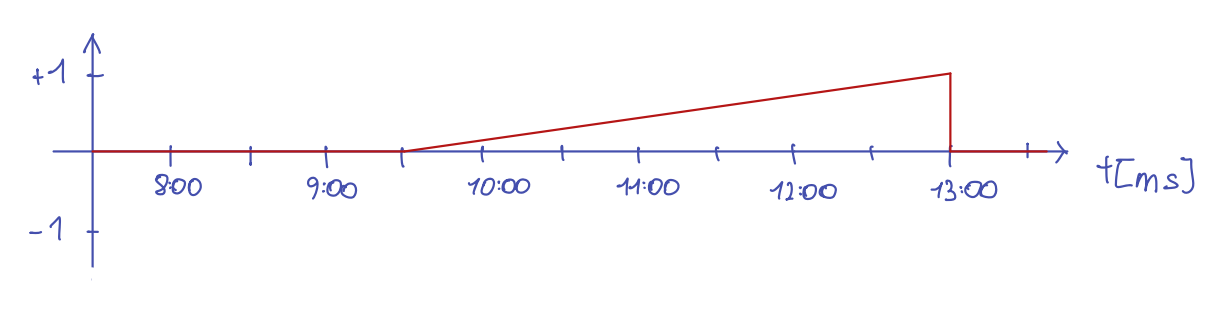
\includegraphics[width=10cm]{images/KA160322/1a.PNG}
  \centering
\end{figure}

\subsubsection{b)}
Es handelt sich um feste Echtzeit, wird die Biet Deadline verpasst kann nicht mehr geboten werde und das
Teil nicht mehr erworben werden.

\subsection{Busse}
\subsubsection{a)}
Erläutern Sie, was man bei PROFInet unter „Jitter“ versteht und wie IRT für einen sehr geringen Jitter
sorgt.

Jitter ist die Variation der Zeit, welche zum Übertragen der Daten benötigt wird. IRT ist vollständig in Hardware
implementiert und priorisiert Echtzeitdaten um sicherzustellen, dass Daten in einem konstanten Zeitrahmen übertragen werden.

\subsubsection{b)}
An einem CAN-Bus sind eine SPS, ein Bewegungsmelder, sowie eine Lampe angeschlossen. Die SPS liest
alle 500 Millisekunden den Bewegungsmelder aus, falls seit dem letzten Auslesen eine Bewegung
detektiert wurde sendet die SPS unmittelbar danach ein Kommando an die Lampensteuerung um eine
Neonröhre einzuschalten. Eine Leseoperation auf dem CAN-Bus dauert 2 Millisekunden, eine
Schreiboperation dauert 1 Millisekunde. Die Neonröhre leuchtet 30 Millisekunden nach Einschalten
auf.\\

Wie viele Millisekunden vergehen maximal zwischen dem Auftreten einer Bewegung und dem
Aufleuchten der Neonröhre?\\
Es vergehen 531ms (Bereich zwischen grünen Strichen)\\
Wie viele Millisekunden vergehen minimal zwischen dem Auftreten einer Bewegung und dem
Aufleuchten der Neonröhre?\\
Es vergehen 33ms (Bereich zwischen grünen Strichen)

\begin{figure}[H]
  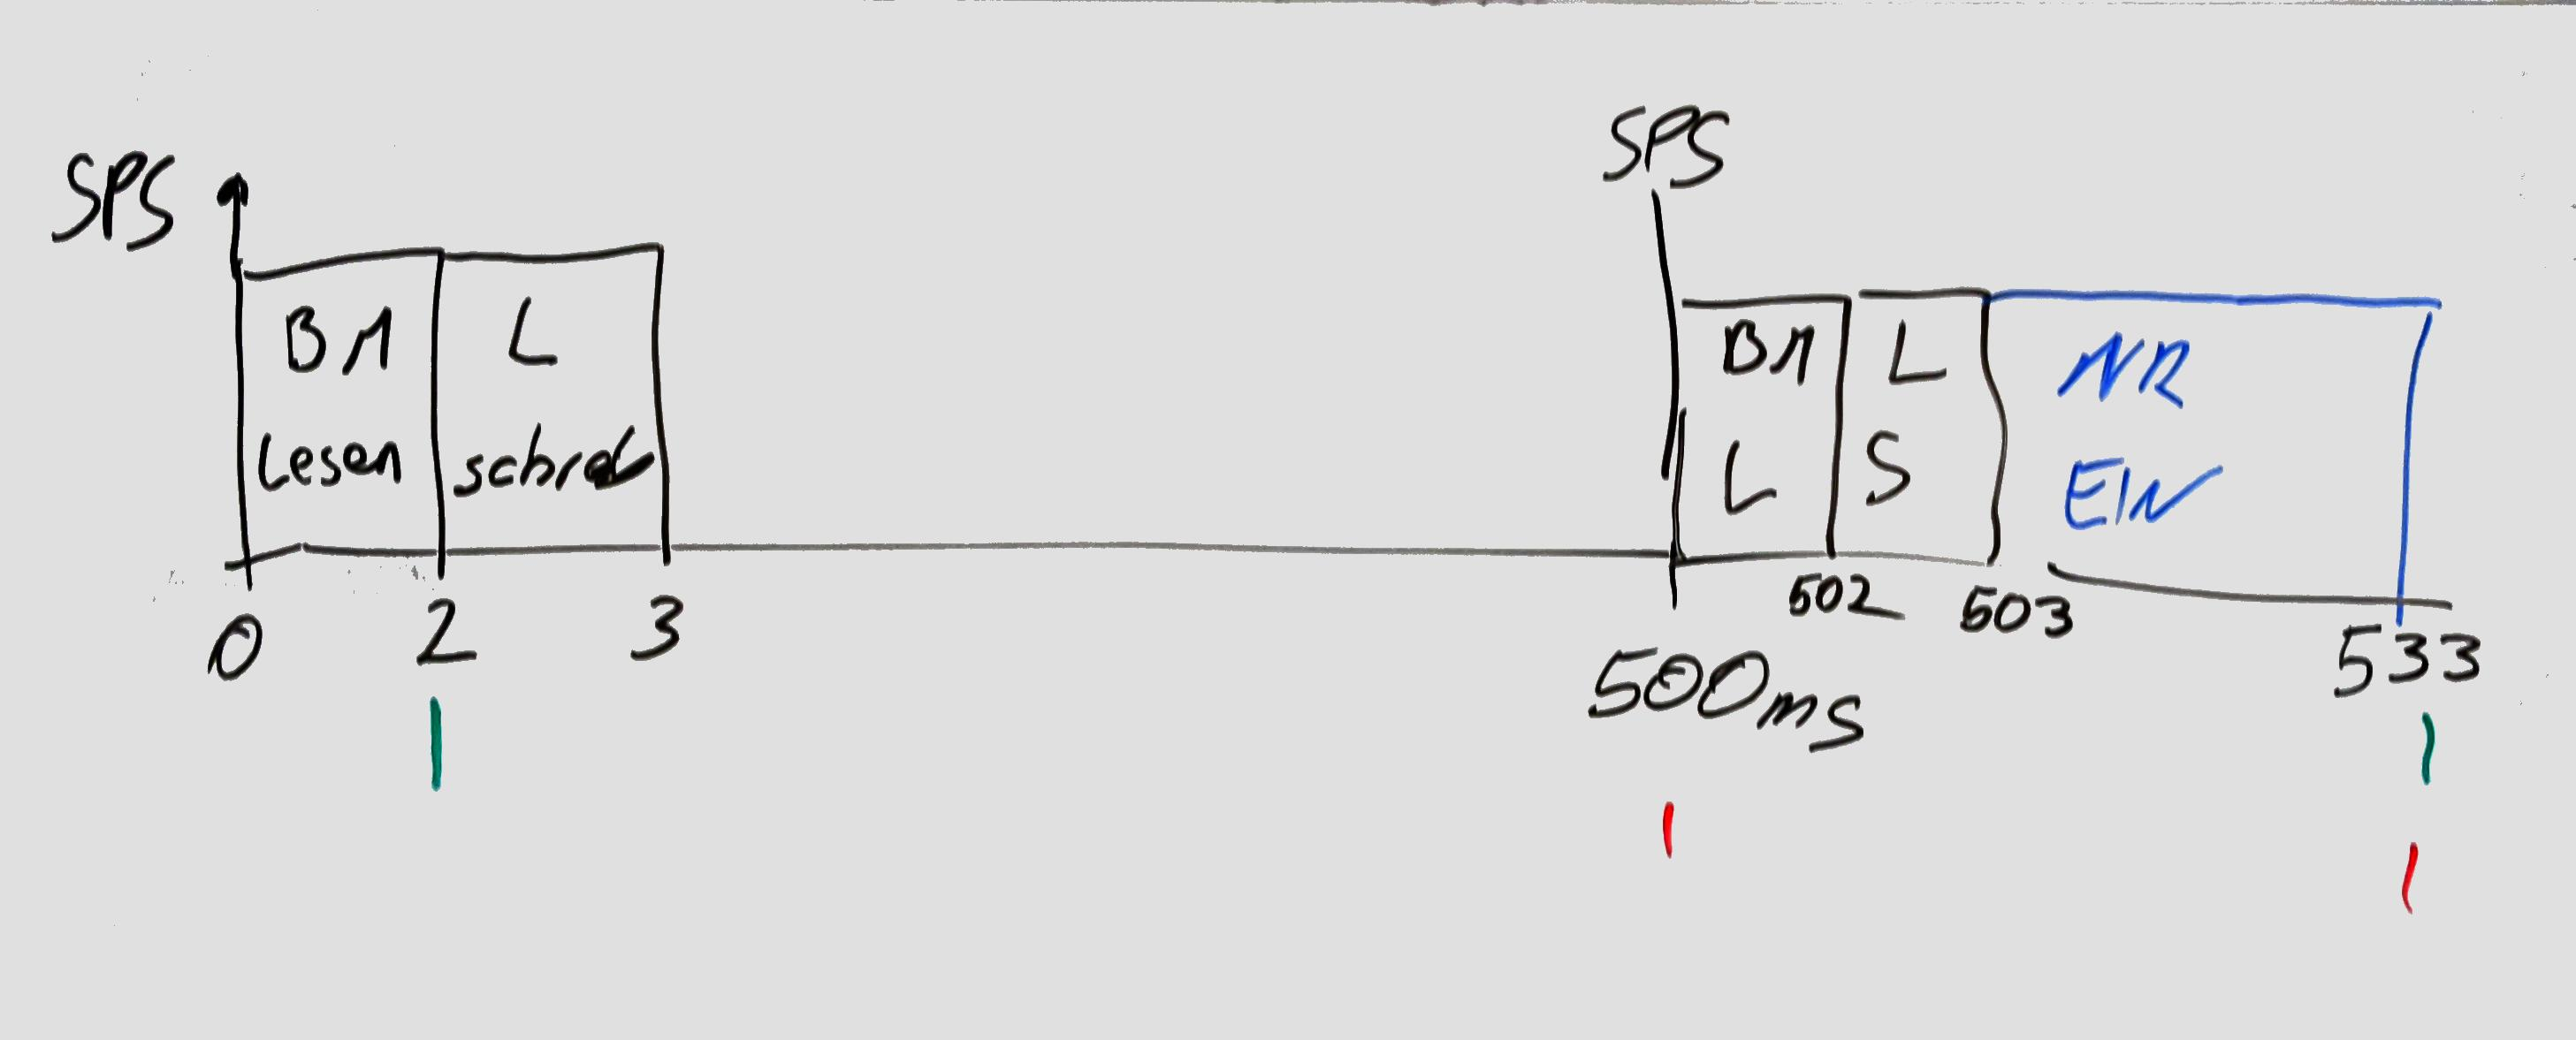
\includegraphics[width=10cm]{images/KA160322/2b.jpg}
  \centering
\end{figure}

\subsection{Echtzeitscheduling}
Gegeben sind folgende drei Tasks:\\
Task1 = (1; 3)\\
Task2 = (2; 5)\\
Task3 = (1; 4)\\
Ein Task ist als Taskj=(Cj; Tj) definiert, wobei Cj die Ausführungszeit (Worst-Case) von Task j und Tj die
Periode von Task j ist. Wir benutzen das Task-Modell aus der Vorlesung, d.h. für jeden Task ist die Periode
identisch mit der Deadline, die Ausführungszeiten der Tasks sind konstant und so weiter. Alle Tasks sind
gleichzeitig zum Zeitpunkt 0 ausführungsbereit.

\subsubsection{a)}
Zeichnen Sie die Ausführung der drei Tasks gemäß RMS bis zum Zeitpunkt 20 in das Diagramm ein: 

\begin{figure}[H]
  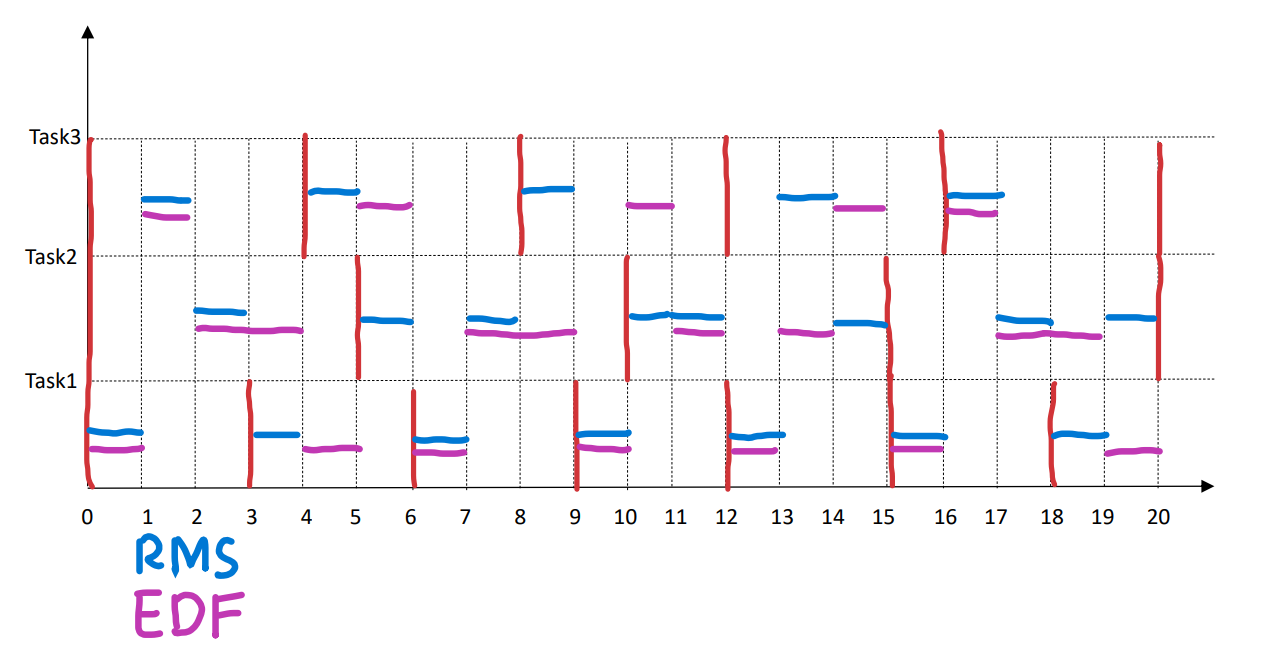
\includegraphics[width=10cm]{images/KA160322/3a.PNG}
  \centering
\end{figure}

\subsubsection{b)}
Werden die Deadlines aller Tasks bis in alle Ewigkeit eingehalten? Begründen Sie!

$U_g(3) = 0.7798$

\begin{equation}
  U = \frac{1}{3} + \frac{2}{5} + \frac{1}{4} = 0.9833 \leq U_g(3) = 0.7798
\end{equation}
Da $0.9833$ nicht kleiner gleich wie $0.7798$ ist, können die Deadlines nicht bis in alle Ewigkeiten eingehalten werden.\\

RMS $U > 1$ nicht schedulebar, bei $U <= 1$ eventuell, $U \ U(n) <= 1$ fix\\
EDF $U > 1$ nicht schedulebar, bei $U <= 1$ fix

\subsection{Taskprioritäten}
\subsubsection{a)}
Definieren Sie den Begriff „Prioritätsinvertierung“.

An einer Prioritätsinversion sind mehrere Prozesse oder Threads mit unterschiedlicher Priorität und eine Ressource beteiligt.
Die Ressource ist durch einen Mutex oder eine Semaphore gelocked.
\subsubsection{b)}
Welche Voraussetzungen müssen erfüllt sein damit eine Prioritätsinvertierung auftreten kann?
Begründen Sie Ihre Antwort!

Ein Task mit niedriger Priorität muss eine Resource locken welche später von einem hoch prioren Task gebraucht wird. 
Da der niedrig priore Task die Resource nicht freigegeben hat kann der hoch priore Task nicht zugreifen und muss warten.

\subsubsection{c)}
Was ist der Unterschied zwischen einer unbeschränkten Prioritätsinvertierung und einer beschränkten
Prioritätsinvertierung?

Bei unbeschränkter Prioritätsinvertierung wird der verdrängte Task nicht mehr gescheduled. Bei beschränkter Prioritätsinvertierung
wird der verdrängte Task nur für eine bestimmte Zeit nicht gescheduled.

\subsubsection{d)}
Erläutern Sie ein Verfahren um die unbeschränkte Prioritätsinvertierung zu vermeiden!

Ressource bekommt ebenfalls eine Priorität, die höher als die der höchstprioren sie nutzenden Task ist.
Nutzt eine Task die Ressource, nimmt sie temporär diese höhere Priorität an. Oder Priority Aging.

\subsection{Statecharts}
Der folgende Programmcode wurde aus einem Statechart generiert. Zeichnen Sie den ursprünglichen
Statechart, tragen Sie auch die Namen aller Zustände sowie aller Ereignisse ein und markieren Sie alle
initialen Zustände so wie in Statecharts üblich!

\begin{lstlisting}
#define Q 1
#define R 2
#define S 3
void main () {
  int state = Q;
  while (1) {
    int a = update_a();
    int b = update_b();
    int c = update_c();
    if (a) {
      state = R;
    } else {
      switch (state) {
        case Q: if (b) { state = S; } break;
        case S: if (c) { state = Q; } break;
        case R: if (b) { state = S; }
                else if (c) { state = Q; } break;
      }
    }
  }
}

\end{lstlisting}
\begin{figure}[H]
  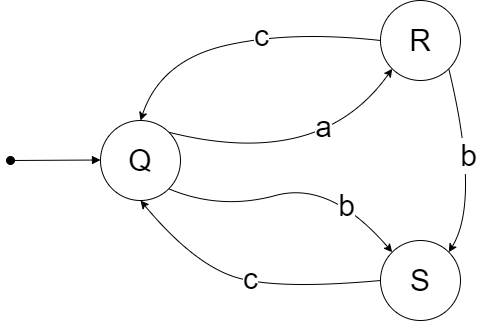
\includegraphics[width=10cm]{images/KA160322/5a.png}
  \centering
\end{figure}

\subsection{Speicherprogrammierbare Steuerung (SPS)}
Geben Sie zu folgendem Strukturierten Text eine Anweisungsliste und einen Funktionsplan an welche die
gleiche Funktion ausführen wie der Strukturierte Text:

\begin{lstlisting}
  IF A AND (B OR NOT C) THEN
    D := TRUE;
  ELSE
    D := FALSE;
  END_IF;
  Timer (IN:=D, PT:=#5s);
  E := Timer.Q;
\end{lstlisting}

\subsubsection{Anweisungsliste (AWL)}
\begin{lstlisting}
  LD B
  ORN C
  AND A
  ST D

  CAL Timer (IN:=D, PT:=T#5s)
  LD Timer.Q
  ST E
\end{lstlisting}

\subsubsection{Funktionsplan (FUP)}
\begin{figure}[H]
  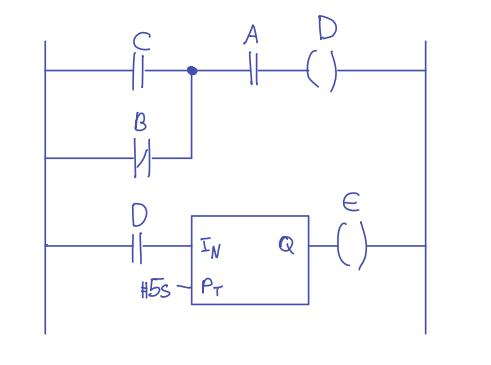
\includegraphics[width=10cm]{images/KA160322/6a.png}
  \centering
  \caption{Funktionsplan}
\end{figure}

\begin{figure}[H]
  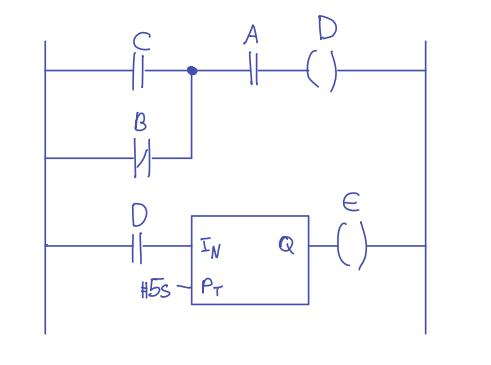
\includegraphics[width=10cm]{images/KA160322/6a.png}
  \centering
  \caption{Kontaktplan}
\end{figure}